%!TEX root = ../Main.tex

\chapter{Assignment 3.2}

\textbf{Create a module (ModuleDouble) with two threads (A, B), one method (A) and four events (A,
	B, Aack, Back) as shown in Figur 1. Thread A notifies event A every 3 ms and thread B notifies
	event B every 2 ms. After notification, the thread waits for an acknowledge (event Aack and Back).
	If acknowledge is not received after a timeout period (A = 3 ms and B = 2 ms) the threads continue
	notifying event A or B. The method A alternates between waiting on event A and B. Use dynamic
	sensitivity in the method by calling next\_trigger() to define the next event to trigger the method.
	Let the method print the current simulation time and the notified events. 
}


For this exercise two threads, a method and four events were created. Below is a snippet code from ModuleDouble.h. 

\section{ModuleDouble.h}
\begin{lstlisting}
#pragma once
#include <systemc.h>
SC_MODULE(ModuleDouble) {

// Events used by used by method.
sc_event A, B, Aack, Back;

// Bool used to keep track of method notified.
bool next_trigger_from_A = true;

SC_CTOR(ModuleDouble)
{
// Threads in module.
SC_THREAD(Thread_A);
SC_THREAD(Thread_B);

// Method
SC_METHOD(Method_A);
// Static sensitivity used to start method. Then overwritten by dynamic sensitivity.
sensitive << A;
// To make sure that method isn't called when module is initialized.
dont_initialize();
}

// Function prototypes.
void Thread_A(void);
void Thread_B(void);
void Method_A(void);
};
\end{lstlisting}


\section{ModuleDouble.cpp}

The implementation of Thread\_A and Thread\_B is showed in the code snippet below. 
Thread\_A notifies event A every 3ms, or when event Aack is notified. 
Thread\_B notifies event B every 2ms, or when even Back is notified. 
 
Method\_A must print out the simulation time and the event notified. To check which event that triggered Method\_A an if-statement is implemented. The if -statement checks a Boolean called next\_trigger\_from\_A. If that Boolean is true, the Event Aack is notified, and the call next\_trigger(B) is used, to change the dynamic sensitivity of the process, so next time its triggered event B is notified. 

\begin{lstlisting}
#include "ModuleDouble.h"
#include <string>
using namespace std;

void ModuleDouble::Thread_A(void)
{
// Notifies event A every 3ms (simulation time).
// Thread is "woken up" if Aack-event is notified.
while (1)
{
A.notify();
wait(3, SC_MS, Aack);
}
}

void ModuleDouble::Thread_B(void)
{
// Notifies event B every 2ms (simulation time).
// Thread is "woken up" if Back-event is notified.
while (1)
{
B.notify();
wait(2, SC_MS, Back);
}
}

void ModuleDouble::Method_A(void)
{
string str;

// Check whether the event that triggered the method was event_A og event_B.
// Write the name of the event to the string, notify the 
// correct acknowledge-event and set up dynamic sensitivity for the other event.
if (next_trigger_from_A)
{
next_trigger_from_A = false;
str = "A";
Aack.notify();
next_trigger(B);

}
else
{
next_trigger_from_A = true;
str = "B";
Back.notify();
next_trigger(A);
}

// Print simulation time and event notified.
cout << "Simulation time: " << sc_time_stamp() << " - Event notified: " << str << endl;
}
\end{lstlisting}


The main.cpp just creates an instance of the ModuleDouble and calls sc\_start(200, SC\_MS); to make it run for 200ms. 
Below is a screenshot of the Console.

\begin{figure}[H]
	\centering
	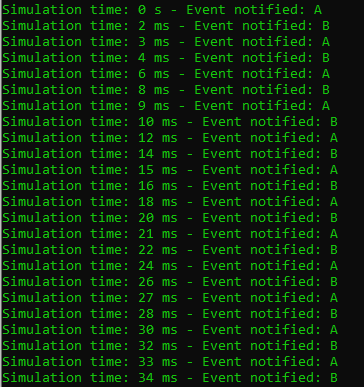
\includegraphics[width=\textwidth]{Images/ConsoleWindow3_2.png}
	\caption{A screenshot of the console}
	\label{fig:ConsoleWindow_3_2}
\end{figure}

